\section{Unmanned Aerial System (UAS)}\label{sec:uas}
In some cases it is necessary to talk about our system as a whole, such that we use it further. The UAS can be seen in Figure \ref{fig:uas} and it is composed of the following:
\begin{itemize}
	\item Drone
	\item GNS
	\item Communications
	\item Survey camera
\end{itemize}

\begin{figure}[h]
	\centering
	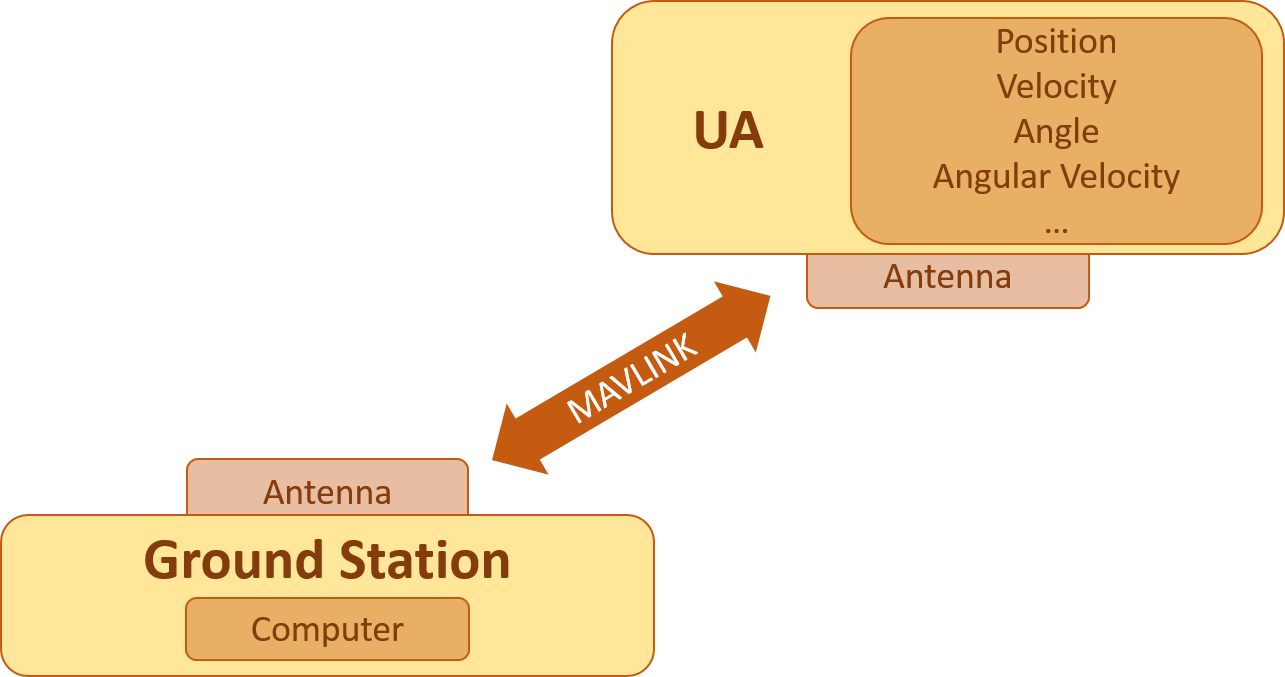
\includegraphics[scale=0.33]{figures/uas.png}
	\caption{Unmanned Aerial System Overview}
	\label{fig:uas}
\end{figure}

In order to have some bounds of the system we can have a look at the drone performances:
\begin{itemize}
	\item 50 km/h - stability at high speeds 
	\item 40 minutes - battery autonomy (30 minutes with payload)
	\item 2400 m - maximum flight altitude (higher if take off from mountain site)
	\item 50 km - maximum radio communication (with directional antennas)
	\item under 1 m - absolute positioning of X-Y GPS
	\item GPS return-to Home (automatically activates when radio link is lost)
\end{itemize}

\subsection{Drone Overview}
			! !	! ! ! ! ! ! ! ! ! ! ! !
! ! ! ! ! ! ! WE NEED SOMETHING HERE ! ! ! ! ! !
			! ! ! ! ! ! ! ! ! ! ! ! ! !

\begin{figure}[H]
  \centering
  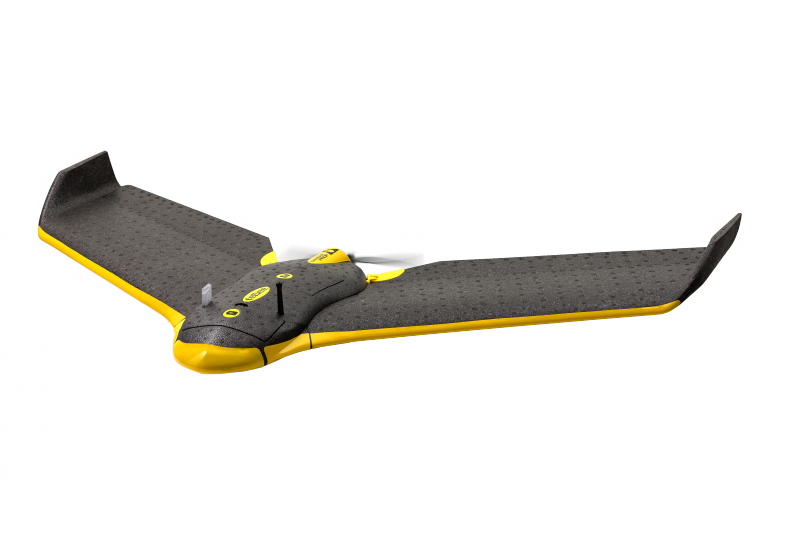
\includegraphics[width=4in]{figures/eBee.png}
  \caption[The professional mapping drone eBee]
   {The professional mapping drone \textit{eBee} \href{https://www.sensefly.com/drones/ebee.html}{(www.sensefly.com)}. Fully autonomous drone to capture high-resolution aerial photos that can transform into accurate 2D orthomosaics \& 3D models.}
\end{figure}

\subsection{GNS Overview}
			! !	! ! ! ! ! ! ! ! ! ! ! !
! ! ! ! ! ! ! WE NEED SOMETHING HERE ! ! ! ! ! !
			! ! ! ! ! ! ! ! ! ! ! ! ! !

\subsection{Antenna Overview}
The antennas used for the GNS and the drone are different by means of weight and size. The preference of using them is based on the application at hand, thus for:
\begin{itemize}
	\item GNS - Parabolic (grid) directional antenna 
	\item Drone - Patch directional antenna
\end{itemize}

A parabolic antenna in an antenna that uses a parabolic reflector and a curved surface to direct the radio waves and its main advantage is that it has a high directivity. This type of antennas are able to produce the narrowest beam widths which allow them to have some of the highest gains.

Parabolic antennas, due to their high gain, are intensively used for carry telephone and television signals between nearby cities. In our specific case, it’s possible to use this property to receive the information provided by the thermal camera through the UAS.

Patch antenna, which is the original type of microstrip, is a low profile antenna that can be mounted on a flat surface and it consists in a rectangular sheet of metal. These antennas are very useful because they are very thin and their directivity varies from 5 to 7 dB.

\begin{table}[h!]
	\centering
	\begin{tabular}{|c||c|c|}
		\hline
		Parameter & GNS & Drone\\ \hline\hline
		Type & Parabolic & Patch\\ \hline
		Polarization & Linear & Linear\\ \hline
		Frequency [GHz] & $2.4$ & $2.4$\\ \hline
		Gain [dB] & $24$ & $14$\\ \hline
		HPBW/$H(^{\circ})$ & $14$ & $45$\\ \hline
		HPBW/$V(^{\circ})$ & $10$ & $45$\\ \hline
	\end{tabular}
	\caption{Table of antennas parameters}
	\label{table:1}
\end{table}

\subsection{Technical Scenario}
As mentioned before we need to assure the maximum distance of communication possible between the GNS and the drone at a certain working frequency:

\begin{equation*}\label{eq:tech_parameters1} 
 	\begin{cases}
 		d_{max} = 50 km	\\
 		f = 2.4 GHz
 	\end{cases}
\end{equation*}

Computing signal wavelength ($\lambda$) for the working frequency stated above:
\begin{equation*}\label{eq:tech_parameters2}
	\lambda = \frac{c}{f} = \frac{3\cdot 10^{8}}{2.4\cdot 10^{9}} 
	        = 0.125 \text{m}
\end{equation*}

Computing the path loss for a distance of 50 kilometers and the signal wavelength:
\begin{equation*}\label{eq:tech_parameters3}
	L = 20\lg\left (\frac{4\pi d_{max}}{\lambda} \right)
	  = 20\lg\left (\frac{4\pi \cdot 50}{0.125\cdot 10^{-3}} \right)
	  = 134 \text{dB} 
\end{equation*}

Computing the output power of the transmitting antenna of 1 Watt:
\begin{equation*}\label{eq:tech_parameters4}
	P_{TX} = 10\lg\left (\frac{1}{10^{-3}} \right)  
	       = 30 \text{dBm}
\end{equation*}


A simplified link budget omitting some losses of the UAS:
\begin{equation*}\label{eq:tech_parameters5}
	P_{RX} = P_{TX} + G_{TX} + G_{RX} - L  
	       = 30 + 24 + 14 - 134 = -66 \text{dBm}
\end{equation*}